\documentclass{beamer}
\def\java{\texttt{Java}}
\def\mytoday{23 November 2016}
\def\mpause{\pause}
\usepackage{pgfpages}\def\mpause{\pause}
%\usepackage{pgfpages}\pgfpagesuselayout{8 on 1}[a4paper,border shrink=1mm, landscape]\def\mpause{}
\usepackage{url}
\usepackage{verbatim}
\usepackage{color}
\usepackage{listings}
\usepackage{code}
\usepackage{textcomp}
%\usepackage{epsfig}
\usepackage{graphicx}

%\usepackage{bm}
\usepackage{beamerthemesplit}
\defbeamertemplate*{footline}{infolines theme}{
\hspace*{2ex}    \insertframenumber{} / \inserttotalframenumber\hspace*{2ex} 
\copyright Manfred Kerber
%   \insertpagenumber{} / \insertpresentationendpage \hspace*{2ex}
  \vskip1ex}

\def\mcolor#1#2{\rule{0ex}{0ex}\color{#1}#2\color{black}{}}
\usetheme{Copenhagen}
%\setbeamercolor{title}{fg=red!80!black,bg=red!20!white}
%\makeatletter % code block to allow custom labels to be cross-ref'ed; see comp.text.tex "customized display labels cross-ref'd"

\begin{document}

\title{MSc/ICY Software Workshop\\
Graphics}

\author[Manfred~Kerber]{\begin{tabular}{ll}
\mcolor{blue}{Manfred Kerber} &   {\tt www.cs.bham.ac.uk/\~{}mmk}\\
\end{tabular}}

\date{\mytoday}

\begin{frame}
\titlepage
\end{frame}

\begin{frame}[fragile]
\frametitle{JFrame}

In the following we will look at packages called AWT Graphics and
Swing for the graphical display.  In order to display objects
graphically in a subclass of \texttt{JPanel},\\
\mcolor{blue}{\texttt{public class NewClass extends JPanel}},\\
we always first create a \texttt{JFrame} of a particular size by


\mcolor{blue}{\texttt{JFrame frame = new JFrame()}}\bigskip


We can set the size and the title of the frame by\\

\mcolor{blue}{\texttt{final int FRAME\_WIDTH = 600;}}\qquad 600 pixels\\
\mcolor{blue}{\texttt{final int FRAME\_HEIGHT = 400;}}\qquad 400 pixels\\
\mcolor{blue}{\texttt{frame.setSIZE(FRAME\_WIDTH, FRAME\_HEIGHT);}}\\
\mcolor{blue}{\texttt{frame.setTITLE("Example frame");}}\\\bigskip


Usually we want the application to terminate when the frame is closed
and want it to be visible:

\mcolor{blue}{\texttt{frame.setDefaultCloseOperation(JFrame.EXIT\_ON\_CLOSE);}}\\
\mcolor{blue}{\texttt{frame.setVisible(true);}}

\end{frame}

\begin{frame}[fragile]
\frametitle{JPanel}

We add to a frame a so-called \texttt{JPanel}.

\mcolor{blue}{\texttt{JPanel panel = new JPanel();}}

On the panel we draw objects by overriding the method\\
\mcolor{blue}{\texttt{public void paintComponent(Graphics g)}}
e.g.
\begin{verbatim}
@Override
public void paintComponent(Graphics g) {
  g.drawRectangle(10,20,200,100);
}
\end{verbatim}
\begin{center}
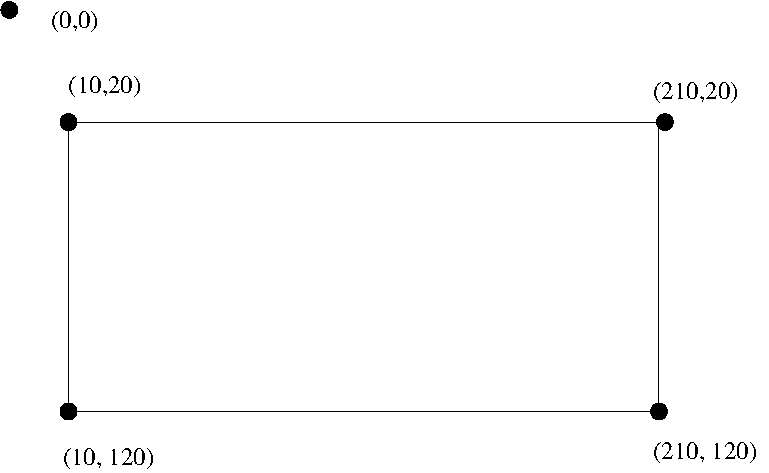
\includegraphics[width=.5\textwidth]{./rec1.pdf}
\end{center}
\end{frame}

\begin{frame}[fragile]
\frametitle{What to Add to a Panel?}

  Note that the dimensions are given in pixels from the left-right
  corner of the frame.

We can draw:

\begin{itemize}
\item outline of a Rectangle \mcolor{blue}{\texttt{drawRect(x, y, width, height)}}
\item filled Rectangle \mcolor{blue}{\texttt{fillRect(x, y, width, height)}}
\item outline of an Oval \mcolor{blue}{\texttt{drawOval(x, y, width, height)}}
\item filled Oval \mcolor{blue}{\texttt{fillOval(x, y, width, height)}}
\end{itemize}

Note that the \texttt{x} and \texttt{y} in case of an oval (ellipse)
give the left uppermost point of the bounding box of the oval (not the
oval itself).\vspace{-0.7cm}

\begin{center}
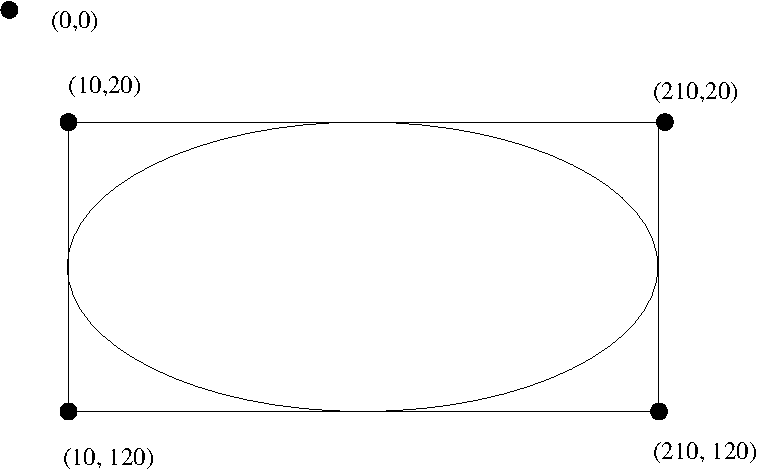
\includegraphics[width=.5\textwidth]{./oval1.pdf}
\end{center}

\end{frame}

\begin{frame}[fragile]
\frametitle{What to Add to a Panel? (Cont'd)}

We can add a line from \texttt{(x0,y0)} to \texttt{(x1,y1)} by adding the line to the body of \texttt{paintComponent}, that is, by
        
\begin{verbatim}
@Override
public void paintComponent(Graphics g) {
   g.drawLine(x0, y0, x1, y1);
}
\end{verbatim}

\end{frame}

\begin{frame}[fragile]
\frametitle{What to Add to a Panel? (Cont'd)}
By setting a font by something like\\
\mcolor{blue}{\texttt{setFont(new Font("Dialog",1,12))}} we can add some text by:\\
\mcolor{blue}{\texttt{g.drawString("Some text added here",10,10)}} at position (10,10).

We can draw arbitrary polygons by specifying the \texttt{x}- and
\texttt{y}-values of the vertices by two arrays:
\begin{verbatim}
        int[] xPoints = new int[vertices];
        int[] yPoints = new int[vertices];
        g.drawPolygon(xPoints, yPoints, vertices);
\end{verbatim}
\texttt{vertices} is the number of vertices of the Polygon.
We can also create a Polygon object by \\
\mcolor{blue}{\texttt{Polygon pol = new Polygon(xPoints, yPoints, vertices)}}

Likewise, \mcolor{blue}{\texttt{drawPolyline}} (does not draw line back to the start).
\end{frame}

\begin{frame}
\frametitle{Adding an image}
We can add an image (in \texttt{paintComponent(Graphics g)}) by
\mcolor{blue}{\texttt{g.drawImage(loadImage(image), xPos, yPos, null)}}
with arguments: an image, the xPosition, the yPosition, and an
ImageObserver not used in our context.
\end{frame}

\begin{frame}[fragile]
\frametitle{Colour}
Some colours are predefined by
 constants such such as BLACK, RED and so on. They can also be
 defined by Color(r,g,b) where r,g,b are values between 0 and
 255. \mcolor{red}{r=red}, \mcolor{green}{g=green}, and \mcolor{blue}{b=blue}. 0,0,0 stands for black, 255,0,0
 for red, 0,255,0 for green, and 0,0,255 blue with other values in
 between.\bigskip

\begin{minipage}{0.43\textwidth}\small
\tt
        {\color[rgb]{0,0,0}BLACK: Color(0,0,0)}\\
	{\color[rgb]{1,0,0}RED: Color(255,0,0)}\\
	{\color[rgb]{0,1,0}GREEN: Color(0,255,0)}\\
	{\color[rgb]{0,0,1}BLUE: Color(0,0,255)}\\
	{\color[rgb]{1,0.784,0}ORANGE: Color(255,200,0)}\\
	{\color[rgb]{1,0.683,0.683}PINK: Color(255,175,175)}\\
	{\color[rgb]{0,1,1}CYAN: Color(0,255,255)}
\end{minipage}\quad
\begin{minipage}{0.53\textwidth}\small
\tt
	{\color[rgb]{1,0,1}MAGENTA: Color(255,0,255)}\\
	{\color[rgb]{0,0,0}{\rule[-0.5ex]{\textwidth}{3ex}}\hspace*{-\textwidth}\color[rgb]{1,1,0}{YELLOW: Color(255,255,0)}}\\
	{\color[rgb]{0,0,0}{\rule[-0.5ex]{\textwidth}{3ex}}\hspace*{-\textwidth}\color[rgb]{1,1,1}{WHITE: Color(255,255,255)}}\\
	{\color[rgb]{0,0,0}{\rule[-0.5ex]{\textwidth}{3ex}}\hspace*{-\textwidth}\color[rgb]{0.75,0.75,0.75}{LIGHT\_GRAY: Color(192,192,192)}}\\
	{\color[rgb]{0.5,0.5,0.5}GRAY: Color(128,128,128)}\\
	{\color[rgb]{0.25,0.25,0.25}DARK\_GRAY: Color(64,64,64)}\\
	{\color[rgb]{0.643,1,0.25}Color(164,255,64)}
\end{minipage}
\end{frame}

\begin{frame}
\frametitle{Many more Methods}

E.g., in \texttt{public void paintComponent(Graphics g)} use\\
\mcolor{blue}{\texttt{g.copyArea(0,0,100,100,300,300)}} [to copy the area in the rectangle from (0,0) to (100,100) to one starting at (300,300)]\bigskip\bigskip

For more methods, see e.g.\\
\mcolor{blue}{\url{http://docs.oracle.com/javase/8/docs/api/java/awt/Graphics.html}}

See, also examples.

\end{frame}
\end{document}


%%% Local Variables: 
%%% mode: latex
%%% TeX-master: "slides"Superclasses
%%% End: 

